\section{Flow: a Home Entertainment Experience over NDN}
\label{sec:components}

% Flow: game experience description
In this section, we describe the design of Flow, a home entertainment experience that leverages NDN to realize a cloud-independent, IoT-supported application. We conclude by summarizing the components of a generalized NDN-IoT framework developed based on this design.
Flow is a prototype of a multi-user ``exploration game'', in which participants navigate and interact with a virtual world rendered in a game engine using a combination of inputs: 
\begin{enumerate}
\item \textit{Indoor positioning}: participants' positions in physical space, detected by indoor positioning (person tracking), modify the virtual landscape;
\item \textit{Wearable sensing}: participants directly control orientation of the environment's virtual camera using gyroscopes connected to  microcontrollers, which can be worn or carried; 
\item \textit{Mobile phone interface}: participants interact with the virtual environment through controls on their smartphone, for example to share social media images in the virtual environment.
\end{enumerate}
In addition to various types of IoT devices and the game engine, the system on which Flow is built also includes an \textit{authentication server} (AS) that performs local trust management.
The AS can be implemented as an app on the owner's smartphone, or a service daemon on a dedicated control hub (e.g., the home router).

\begin{figure}[!t]
\centering
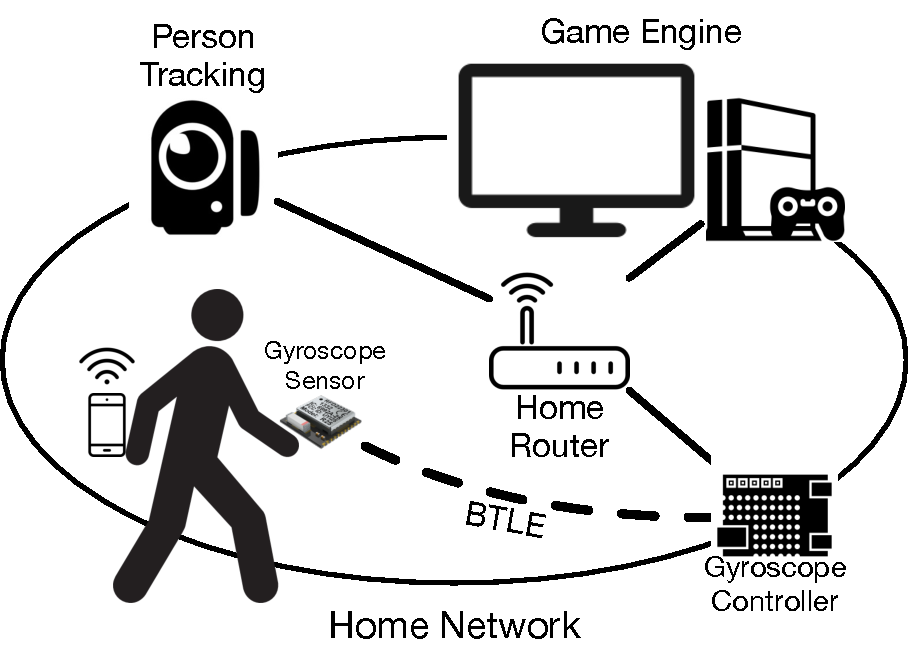
\includegraphics[width=0.9\columnwidth]{flow-home-deployment.pdf}
\caption{Typical deployment of the Flow home entertainment experience.}
\label{fig:flow-deployment}
\end{figure}

% Flow features: cloudless, security, an integrated solution with different types of devices and sensing
%Flow adopts a cloudless architecture, and uses the NDN protocol stack to connect hardware with varying capabilities, as well as secure a diverse range of sensing data. The rest of this section introduces how this is achieved from the perspectives of namespace, bootstrap and trust relationship, and device discovery using synchronization.

Figure~\ref{fig:flow-deployment} shows a typical deployment scenario of Flow in a home network.  NDN interconnectivity between different components is supported over Ethernet and Wi-Fi, through the home Wi-Fi router in a hub-and-spoke topology. 

Sensor devices with limited networking capability (e.g., the gyroscope in Fig.~\ref{fig:flow-deployment}) may be bridged via a helper device.
We assume all devices can reach each other over NDN, which is trivial in a hub-and-spoke topology.\footnote{A routing protocol may be required if a sensor mesh topology is deployed inside the home network.}

\subsection{Naming and Identity}
\label{sec:naming}

% Design: namespace
In Flow, data from the IoT \textit{things} used by the application are named using three namespaces:
\begin{itemize}
\item \emph{Application namespace}: a local namespace for publishing and accessing application data, e.g., gyroscope readings needed to control the environment; 
\item \emph{Device namespace:} a local namespace for publishing device identity certificates and metadata;\footnote{Device metadata could include information about devices and their capabilities as well as bindings to application names.}
\item \emph{Manufacturer namespace}: a global namespace created by the IoT device vendors and for trust bootstrapping.
\end{itemize}


Fig.~\ref{fig:flow-namespace} shows an example of the Flow namespace.  In addition to these three namespaces which names devices, things and their data, note the \textit{discovery} branch under the local root prefix, which is used for device rendezvous and for application prefix discovery. Details of its functionality are described later.


\begin{figure*}[!t]
\centering
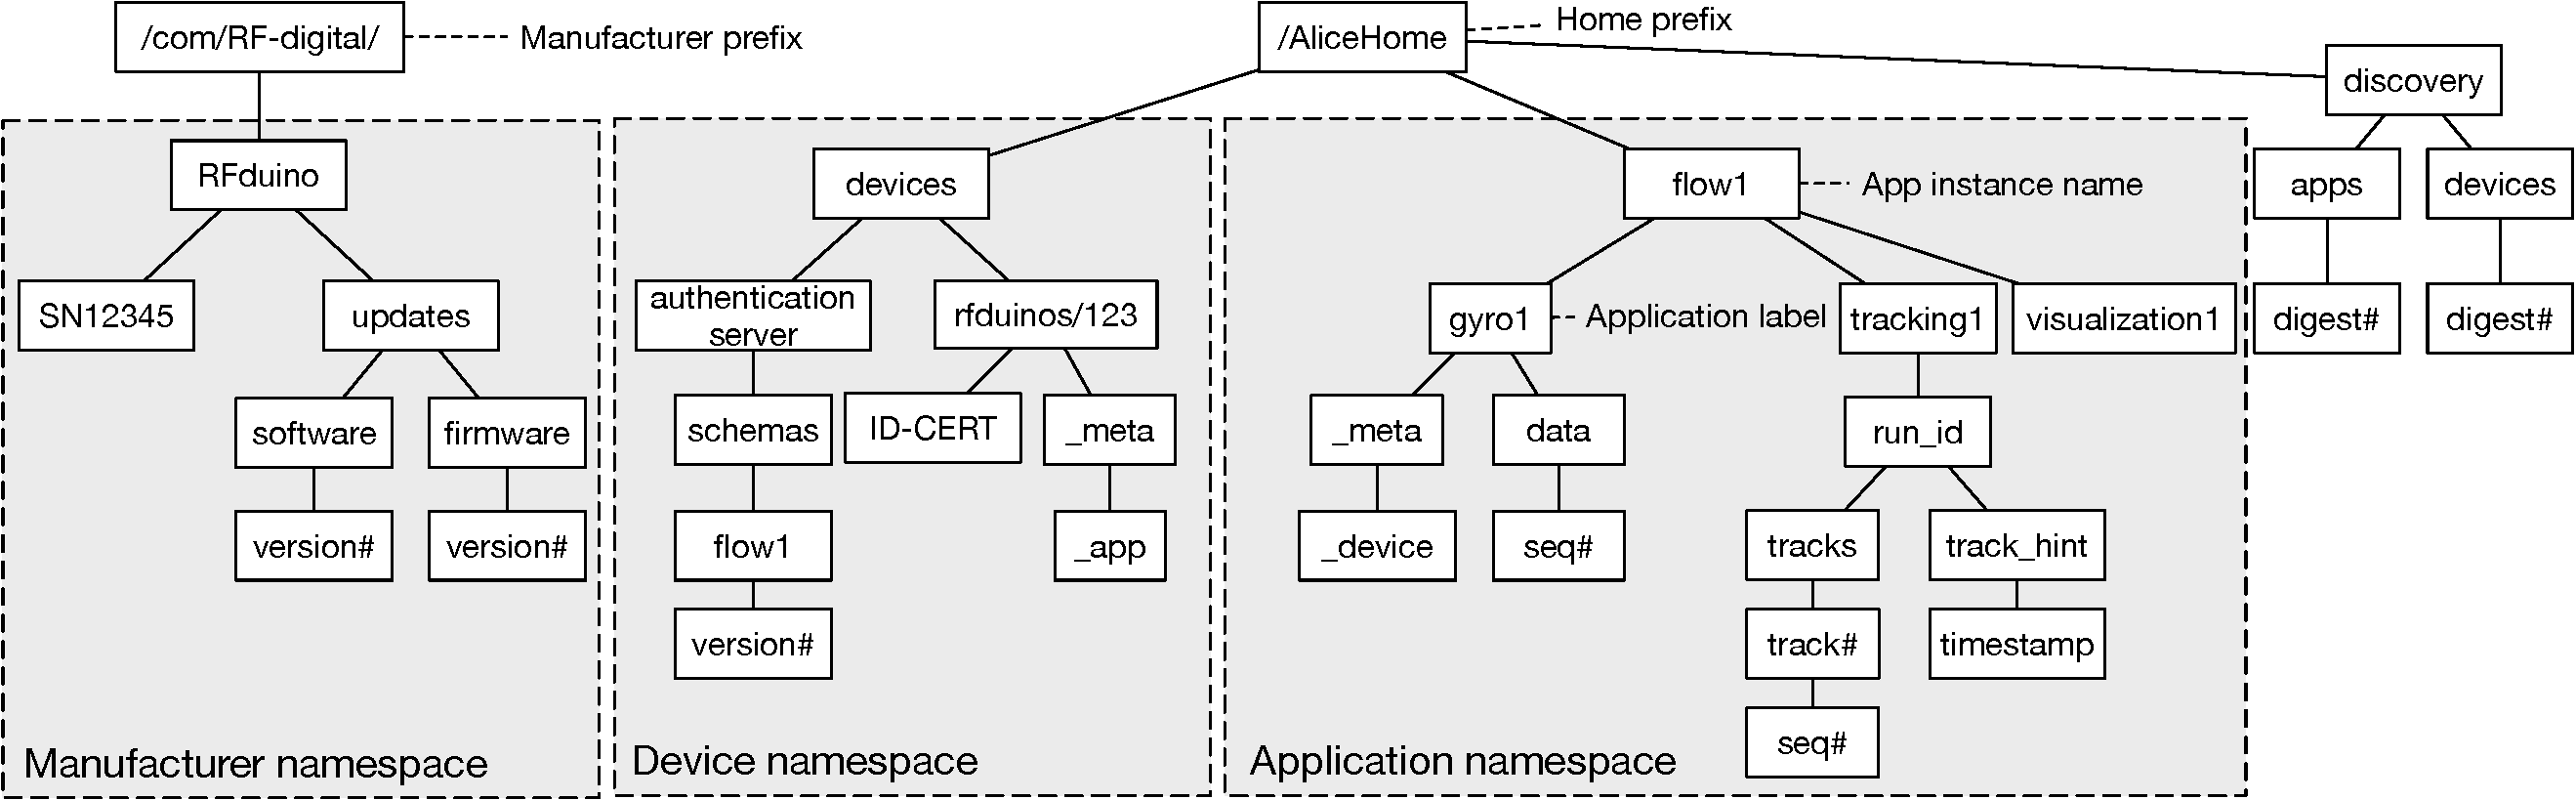
\includegraphics[width=0.95\textwidth]{flow-namespace.pdf}
\caption{Example namespace within the home environment where Flow is deployed.}
\label{fig:flow-namespace}
\end{figure*}

The device and application namespaces both have as their root a home prefix that is either context-dependent (e.g., \ndnName{/AliceHome} as in Fig.~\ref{fig:flow-namespace}) or globally reachable (e.g., \ndnName{/att/ucla/dorm1/301}).

The application namespace starts with a unique instance name (e.g., \ndnName{/AliceHome/flow1}) created by the application at installation. 
Data produced by each component is named under an application label configured by the developer (e.g. \ndnName{/AliceHome/flow1/tracking1}). The application label also contains a metadata subtree containing the device name that serves this data (e.g. \ndnName{/AliceHome/flow1/tracking1/_meta/_device}).

Devices publish their local identity certificates under the device namespace (e.g., \ndnName{/AliceHome/devices}).
They also publish metadata (profile) information in the \ndnName{_meta/_app} branch under the device identity prefix to list the application data prefixes they are publishing under. 
The device namespace of an AS also contains the trust schema of currently active applications. 
Schema and trust relationship details are described later in this section.
%JB: Should reference anything in 2016 paper? 

The manufacturer namespace falls under vendor-specific prefixes that are independent from the home network's local prefix.  We envision that manufacturers will have globally unique names for their products used during  bootstrapping, over-the-air updates, and similar processes. 
Manufacturers publish their own certificates under this globally unique prefix so that the devices can authenticate the data coming from the vendors such as software/firmware updates and service notifications.\footnote{Reachability of data in this prefix is not addressed here but can be accomplished through encapsulation supported by the home router, for example.}
In the research example of Flow, all devices are configured with vendor-provided identity names and profiles in their initial provisioning, before being connected to the home network. These are used for device onboarding.

\subsection{Trust Management}
\label{sec:trust-management}

Flow demonstrates a multi-step process for trusting new devices in a home IoT network and enabling their data to be used in an application.  First, a device is assigned a device-level name and added to the trust hierarchy for things in the home. Then, it is configured with one or more application-level names for its data, and these names are added to application trust hierarchies. Finally, the device is configured to respond to requests in application namespaces. 

%The first step of introducing a new device or user to the Flow system is to establish the trust relationship between the device/user and the existing entities in the system.
The authentication server acts as the trust anchor. It can be coordinated with but does not depend on a remote cloud services.
While the devices and users may have public identities outside the home environment, they all need to obtain local identities that are certified by the AS before they can start interacting with other local entities.\footnote{The public identities may be used to assist the onboarding process, but will not be required for local communication once the initial configuration has finished.
For example, a new user can authenticate with the AS using her public identity (e.g., OpenID or Google/Facebook account) before creating her local identity that is used solely by the home environment.}

The process of establishing a trust relationship between a new device and the home through the AS is similar to the Bluetooth pairing process.
To bootstrap a new device, the user---or a configuration application on his/her behalf---provides a shared secret and a local device name.  The shared secret may be a device barcode, identity communicated by NFC, or simply a PIN number. 
The AS sends a command Interest to the device, signed using a key derived from the shared secret, to ask that it generate a public/private key pair associated with the device's new name on the local network.  The device replies with a Data packet containing an identity certificate request, also signed by the shared secret.
The AS generates the identity certificate based on this request.  The device, now part of the trust hierarchy, can advertise its services or participate in an application over the local network.
This process is illustrated in Fig.~\ref{fig:flow-bootstrap}.
If the device has been issued a public identity certificate by its vendor, the AS may optionally authenticate its public identity, e.g., by asking the device to sign an AS-generated challenge.


\begin{figure}[!t]
\centering
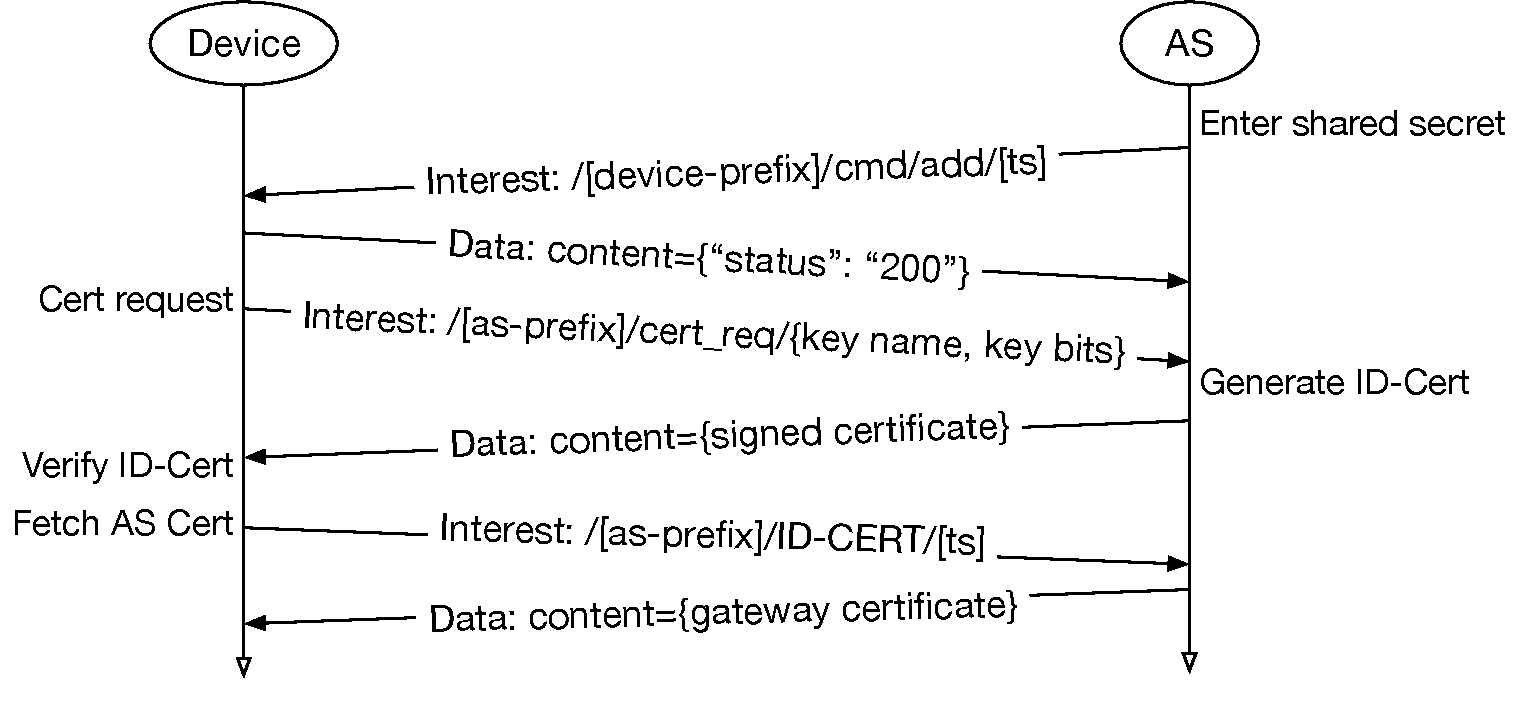
\includegraphics[width=0.95\columnwidth]{add-device-sequence.pdf}
\caption{Bootstrap trust relationship for new device.}
\label{fig:flow-bootstrap}
\end{figure}

Applications like Flow are ``installed'' in a similar way to devices, with the AS signing both identity certificates and trust schema for the application.  The application's trust schema  expresses \textit{what devices identities are authorized to publish under what application prefixes} and is published as a normal Data object on the local NDN network.  For example, in Fig.~\ref{fig:flow-namespace} \ndnName{flow1} is a specific Flow instance and \ndnName{schema} branch contains the trust schema of this instance.
The schema name includes a monotonic version number at the end, so when there is a change in the schema a newer version is published.
The technical details of how to specify a trust schema are described in~\cite{trust-schema}.
% Other device names in the example include an ``RFduino'' device, which in ``flow1''publishes for the gyroscope ``gyro1'' that it's physically connected to. Under a device name a ``\_meta'' branch is introduced, in which the device can list under what application prefixes it's publishing. Two other subsystems of the game, person tracking (``opt1'' branch) and visualization (``unity'' branch) are featured in the example namespace.

%Applications like Flow can request that devices publish data under application-level namespaces by issuing command Interests to them.   The device evaluates the request according to the available trust schema. 

% Design: trust - application producer authorization
When a device that produces data is installed, it sends a command Interest to the AS that includes the application prefix it intends to publish under and its own local identity.
If the request to publish data in the home network is granted, the AS will update the trust schema with the authentication rules for data published by this device. The rule binds a device identity with the application prefixes it's authorized to publish under.\footnote{This binding addresses potential collision in application labels--for example, by default the AS does not authorize a second device to publish under an application namespace claimed by another.}
Schematized trust enables fine-grained control over what devices can publish what data for which application instances. Consumer devices fetch the latest trust schema over the network via NDN and follow the rules to authenticate the data packets published in the network.
The producer authorization process, as well as an example of the resulting trust relationship, is shown in Fig.~\ref{fig:flow-app-authorization-trust-relationship}, in which the AS signs a device identity, and the device signs a piece of application data it publishes.

\begin{figure}[!t]
\centering
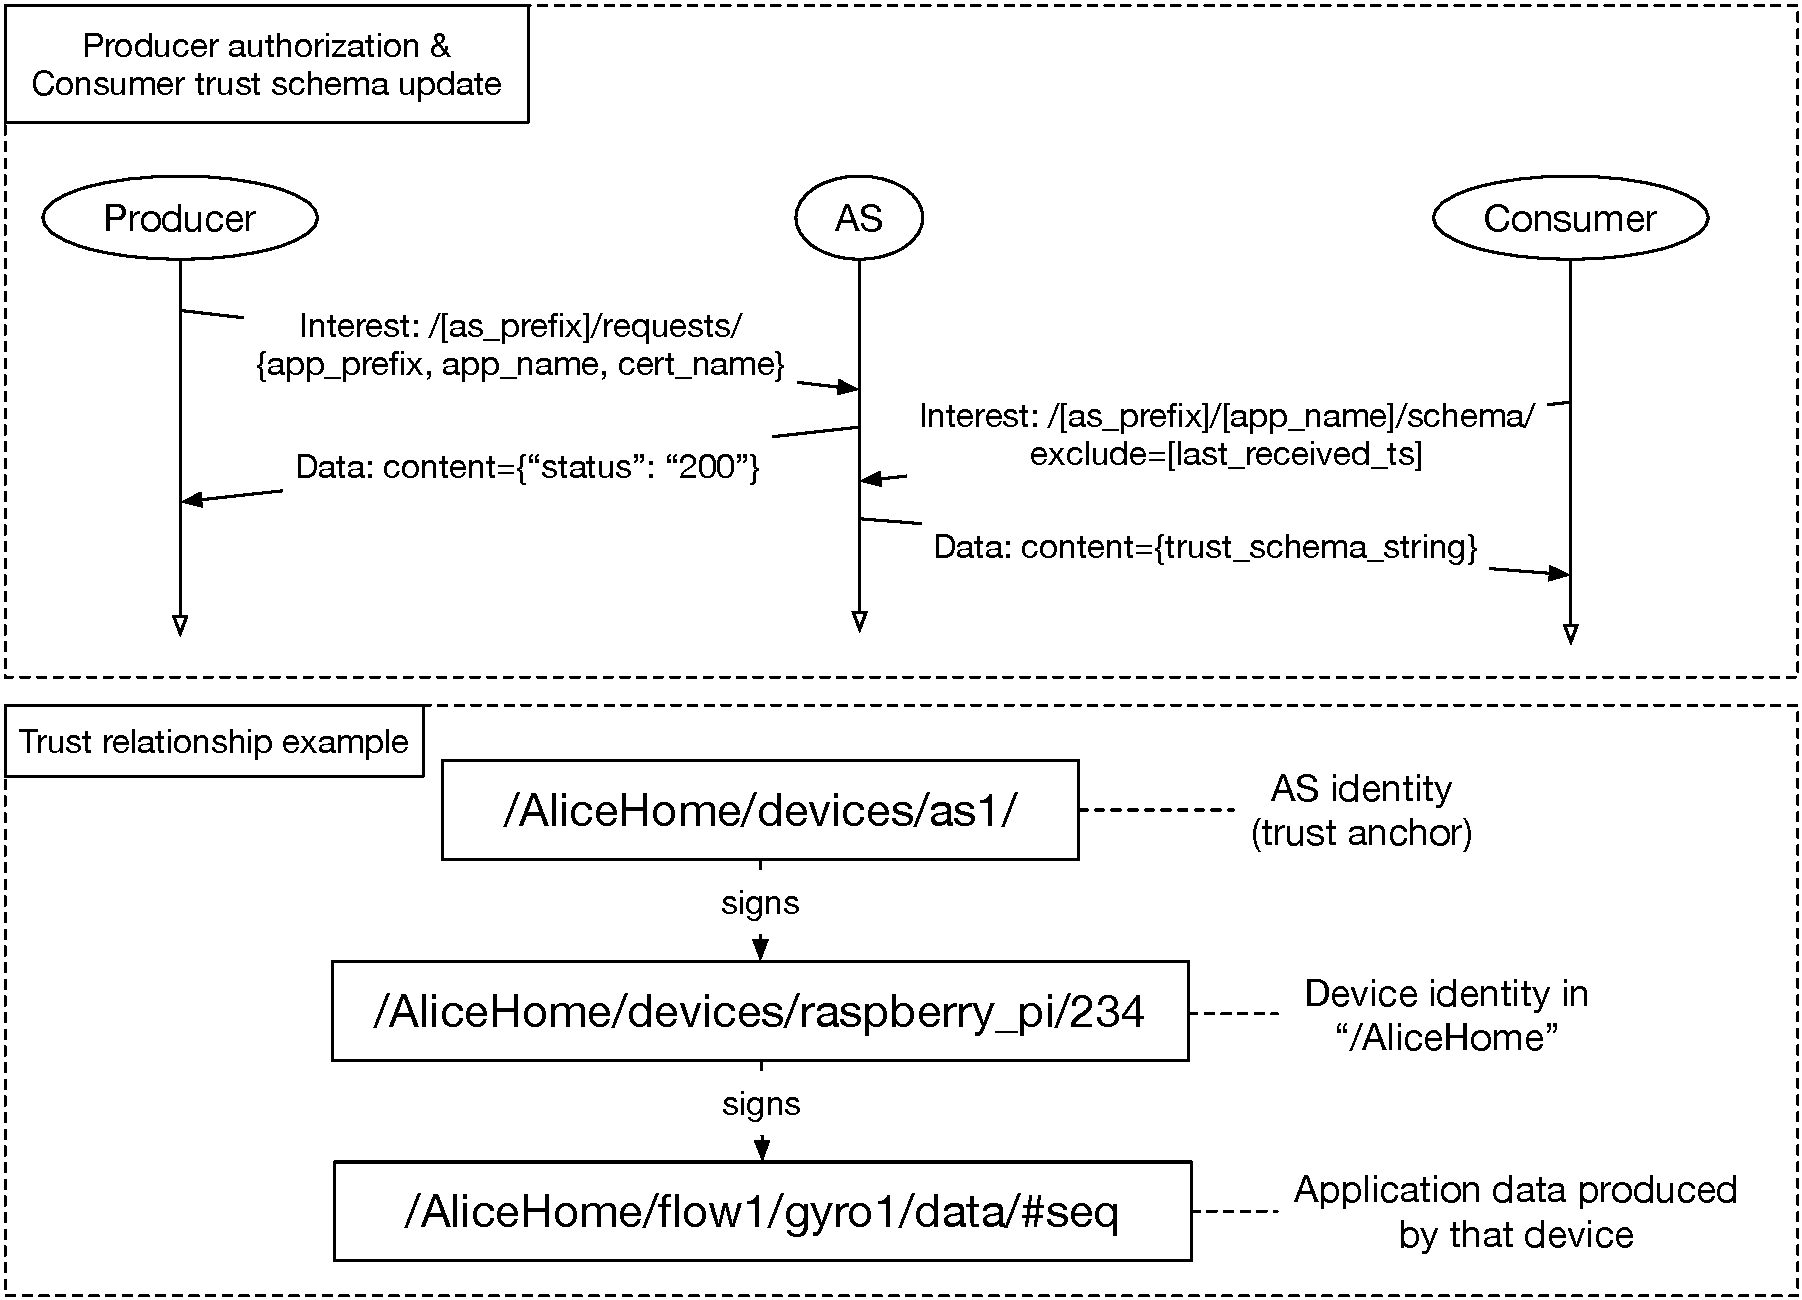
\includegraphics[width=0.95\columnwidth]{authorize-producer-consumer.pdf}
\caption{Schematized trust between producers and consumers.}
\label{fig:flow-app-authorization-trust-relationship}
\end{figure}


\subsection{Rendezvous}
\label{sec:rendezvous}

% Design: discovery (chronosync recovery)
%Each subsystem in Flow needs to learn the application names of other subsystems in order to communicate with them. For this purpose device discovery is introduced. Discovery exchanges messages in ``/home/devices/discovery'' namespace as shown in Fig.~\ref{fig:flow-namespace}, similar to ChronoSync's \cite{chronosync}, a digest of this device's currently known names is attached to the interest name. Receivers of this interest, upon seeing a different digest, will reply with its own set of names. Differing from the suggestion in \cite{ndn-iot}, This synchronization-based discovery is introduced so that any device in the home can help answering a discovery interest, and the controller, after registering the devices and serving required certificates, can stay offline.

Flow also demonstrates a name-based, distributed rendezvous mechanism for devices and applications to discover each other over NDN.
As described in the previous section, The key idea is to synchronize the set of device and application names (called the \textit{rendezvous dataset}) across nodes in the network that are interested in learning about them.
The synchronization process utilizes the decentralized and serverless ChronoSync~\cite{chronosync} protocol to effectively synchronize prefixes of active devices under the home entertainment \ndnName{/AliceHome/discovery/devices} namespace.
% When a device receives a digest different from its own, it replies with a Data packet containing its own set of names.
% Recipients of these replies merge the received dataset with their own local ones.
% Eventually all participating devices will reach agreement about the rendezvous dataset, provided that the configuration changes more slowly than the necessary messages can be exchanged. %system is able to stay in a stable state with no frequent configuration changes.
% This protocol does not require assistance from a central server either locally or remotely.

Name discovery is performed independently on each device by lookups in the local copy of the rendezvous dataset.
% JB: How? Is this an API call? 
Once an application obtains the name prefix of the target device or application, the devices can follow the namespace structure described in~\ref{sec:naming} to construct Interests for fetching the certificates and metadata, which will bootstrap high-level service communication.

%%  JB:  I don't understand this section - seems like it should be rewritten in the context of the IOTDI paper? 

\subsection{Generalizing IoT functionality in NDN}

Through the design of Flow, we explored how to use NDN to provide the functionality discussed in section~\ref{sec:cloud-iot} without reliance on any cloud services, and generalized it in a framework called \textit{NDN-IoT}, which provides the following features: 

\begin{itemize}

\item \textit{Identity, authentication and authorization}: each device in NDN-IoT possesses two identities: a manufacturer-given name used before and during device onboarding, and a local device name used afterwards. NDN-IoT implements mechanisms described in sections~\ref{sec:naming} and ~\ref{sec:trust-management} for naming, data authentication and device authorization. 
% Repetition and no close connection...

\item \textit{Rendezvous and resource discovery}: nodes in NDN-IoT find the name prefixes of other devices, applications and services in \textit{discovery} namespace via distributed dataset synchronization, and then uses discovered names to fetch devices and applications data, or invoke services in the local system. 
% Repetition of the same thing in the last paragraph of Rendezvous

\item \textit{Device management}: NDN-IoT performs device onboarding and software updates in manufacturer namespace, and device monitoring in device namespace. 
% More non-trivial things to say about this?

\item \textit{Application data messaging}: NDN-IoT provides application-level pub-sub under two types of namespace abstractions. The framework pipelines interest for data named in a \textit{sequence number namespace} (e.g. \ndnName{/AliceHome/flow1/gyro1/data/[sequence_number]}), or keeps outstanding interest for data named in a \textit{timestamp namespace} (e.g. \ndnName{/AliceHome/devices/pc1/_status/[timestamp]}).

\item \textit{Gateways to external network and services}: the local IoT system can request data from the global Internet using their public names, meanwhile its local data can be made available to the public Internet by using a globally reachable name prefix, or having a gateway device that uses data named under a globally reachable prefix to encapsulate data from the local system (e.g. \ndnName{/att/ucla/dorm1/301/flow1/gyro1/data/1} $\rightarrow$ \ndnName{/AliceHome/flow1/gyro1/data/1}).

\end{itemize}

